% This is what ChatGPT came up with for Figure 3 in the Metcalfe + Boggs Paper

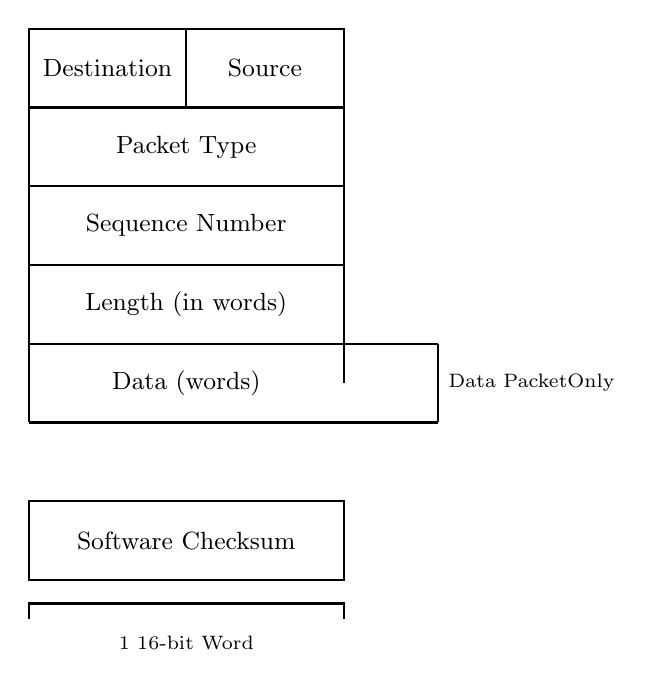
\begin{tikzpicture}[
  font=\sffamily,
  thick,
  % For quick coordinate adjustments, each "word" is 4 cm wide:
  x=4cm,
  % Each row is 1 cm high:
  y=1cm
]

% We will stack rectangles downward (negative y).
% The top left corner of the top row is (0,0).

% 1) Top row: Destination (left half), Source (right half)
\draw (0,0) rectangle (1,-1); % Entire top row is 1 "word" wide in x-coords
\draw (0.5,0) -- (0.5,-1);    % Subdivide into two half-words
% Labels:
\node[align=center, font=\small] at (0.25,-0.5) {Destination};
\node[align=center, font=\small] at (0.75,-0.5) {Source};

% 2) Packet Type row
\draw (0,-1) rectangle (1,-2);
\node[font=\small] at (0.5,-1.5) {Packet Type};

% 3) Sequence Number row
\draw (0,-2) rectangle (1,-3);
\node[font=\small] at (0.5,-2.5) {Sequence Number};

% 4) Length (in words) row
\draw (0,-3) rectangle (1,-4);
\node[font=\small] at (0.5,-3.5) {Length (in words)};

% 5) Data (words) area.
%   We'll show it as partially open at the bottom to suggest variable length.
%   Top line from y=-4 to y=-5, no bottom line to the next box.
\draw (0,-4) -- (1,-4) (0,-5) -- (1,-5); % horizontal lines
\draw (0,-4) -- (0,-5); % left vertical
\draw (1,-4) -- (1,-4.5); % partial right vertical
\node[font=\small] at (0.5,-4.5) {Data (words)};
% "Data Packet Only" bracket on the right
\draw (1,-4) -- ++(0.3,0) 
      (1,-5) -- ++(0.3,0);
\draw (1.3,-4) -- (1.3,-5);
\node[font=\scriptsize, right] at (1.3,-4.5) {Data Packet\\Only};

% 6) Software Checksum row (below data).
%   For simplicity, place it two rows below, i.e. from y=-6 to y=-7
\draw (0,-6) rectangle (1,-7);
\node[font=\small] at (0.5,-6.5) {Software Checksum};
% Optionally draw a horizontal line at y=-5 or -5.5 to “close” the data region:
% \draw (0,-5.5) -- (1,-5.5);

% “1 16-bit Word” bracket at the very bottom
%   We draw a bracket from x=0 to x=1 at y=-7.5, then label underneath
\draw (0,-7.5) -- (0,-7.3) -- (1,-7.3) -- (1,-7.5);
\node[font=\scriptsize] at (0.5,-7.8) {1 16-bit Word};

\end{tikzpicture}


